\subsection{Fonctionnement de l'application}

Cette section présente le fonctionnement global de l'application, afin de mieux cerner le sujet sur lequel nous avons travaillé. Il faut cependant préciser que ce n'est pas sous cette forme que nous avons reçu le projet, il ne fonctionnait que partiellement, la version présentée ici est la version finale post-TER.

\begin{figure}[!h]
\centering
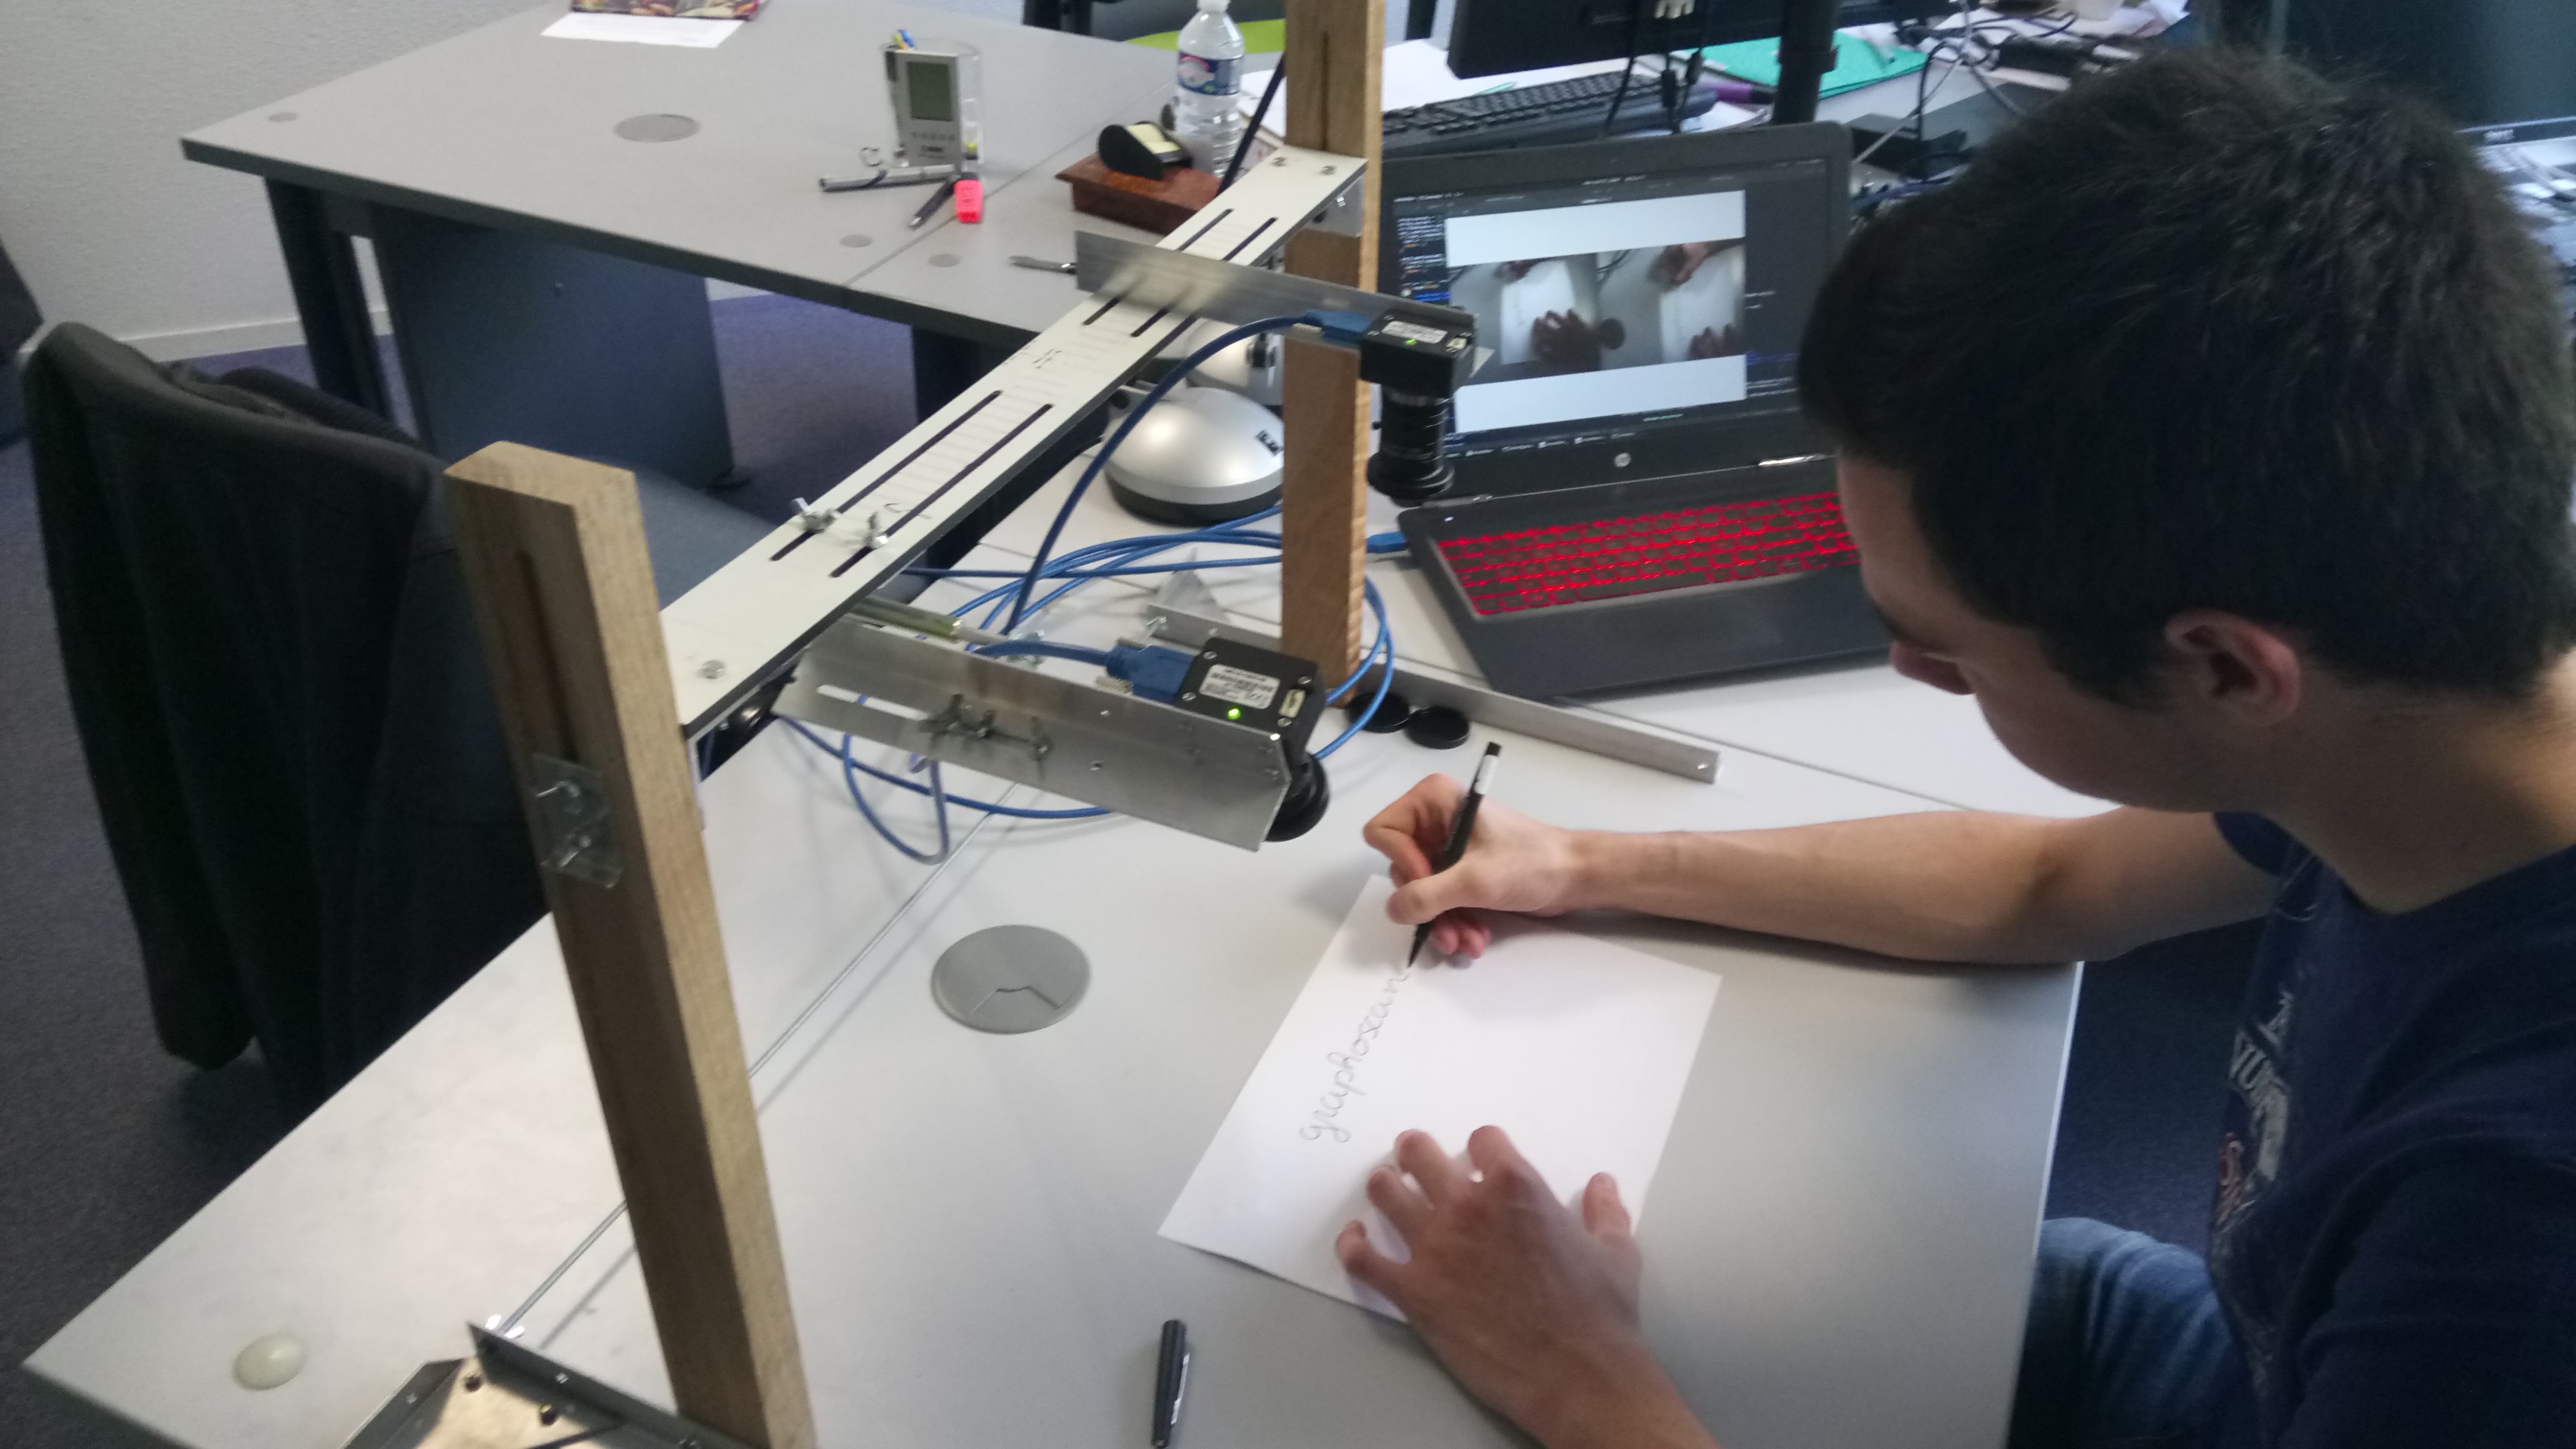
\includegraphics[scale=0.08]{Modules/Picture/Utilisation.png}
\caption{Ecriture et acquisition}
\label{utilisation}
\end{figure}

Le dispositif montré sur la figure \ref{utilisation} nous permet de capturer les vidéos en direct. Ces deux vidéos sont enregistrées sur ordinateur, pour pouvoir faire de la stéréo : on encode les images en même temps pour avoir exactement les mêmes frames au même moment. On applique ensuite des paramètres d'undistortion pour lisser les bords de l'image. En effet, la caméra ayant un grand angle, l'extérieur de l'image est déformé, ce qui peut apporter des problèmes lors de la reconstruction 3D.

Une fois les deux vidéos récupérées, on peut lancer la reconstruction. La première étape est de retrouver l'écriture sur l'image, pour cela différentes méthodes sont disponibles. On peut par exemple faire du tracking. Après avoir sélectionné une zone d'intérêt grâce à un ROI (Region Of Interest) selector (figure \ref{ROI} ), on essaye de suivre le mouvement. Il suffit d'enregistrer les coordonnées du centre du point pour retrouver le mouvement dessiné (figure \ref{tracking} ).

La seconde technique est celle du HOG (Histogramme de gradient orienté) qui permet de détecter des formes dans une image. Ce qui donne au départ une image comme sur la figure \ref{HOGSale}, et après nettoyage \ref{HOGPropre}.

L'une ou l'autre de ces techniques peuvent être utilisées pour avoir une suite de coordonnées correspondant au dessin de l'écriture. Une fois que ces deux coordonnées sont récupérées, il existe des fonctions dans OpenCV pour faire des points 3D à partir de points 2D. Il faut pour cela récupérer les paramètres extrinsèques (matrices de rotation et vecteurs de translation, pour passer du repère lié à l'espace de travail au repère lié à la caméra) de la caméra.

Une fois que les coordonnées sont récupérées par l'une ou l'autre méthode, une fonction nous permet de rajouter deux points entre chaque coordonnée pour fluidifier la ligne. Ces coordonnées sont ensuite interprétées par OpenGL pour permettre de les afficher dans un repère en trois dimensions (figures \ref{3D1} et \ref{3D2} ).


\begin{figure}[htb]
\includegraphics[width=\textwidth]{Modules/Picture/roi}
\caption{ROI selector}
\label{ROI}
\vspace{30px}
\includegraphics[width=\textwidth]{Modules/Picture/tracking}
\caption{Reconnaissance avec le tracking}
\label{tracking}
\end{figure}

\newpage

\begin{figure}
\includegraphics[width=\textwidth]{Modules/Picture/hog}
\caption{HOG brut}
\label{HOGSale}
\vspace{30px}
\includegraphics[width=\textwidth]{Modules/Picture/hog_propre}
\caption{HOG nettoyé}
\label{HOGPropre}
\end{figure}

\newpage

\begin{figure}
\includegraphics[width=\textwidth]{Modules/Picture/3d_1}
\caption{Image 3D - 1}
\label{3D1}
\vspace{30px}
\includegraphics[width=\textwidth]{Modules/Picture/3d_2}
\caption{Image 3D - 2}
\label{3D2}
\end{figure}

\clearpage



\subsection{Langages et frameworks utilisés}

Le programme en lui-même est entièrement réalisé en C++, et différentes bibliothèques graphiques sont utilisées dans ce projet pour le traitement du flux vidéo, dans le but de faire du tracking sur le résultat, comme OpenGL et OpenCV. OpenGL est utilisé pour la reconstruction du mouvement de la plume en 3D, tandis qu'OpenCV est plus utilisé pour le traitement de l'image, notamment toutes les opérations faites dessus. De plus, Matlab est utilisé pour effectuer diverses opérations mathématiques sur les images, comme par exemple pour la calibration originelle servant à l'alignement pour la stéréo, ainsi que pour l'enlèvement de la distorsion. En effet, comme les caméras ont un grand angle, les éléments sur le bord de l'image sont courbés, il faut donc les remettre droits pour pouvoir travailler dessus.

\subsection{Fonctionnalités déjà implémentées}

Le programme tel qu'il nous a été fourni dispose de plusieurs fonctionnalités élémentaires permettant son bon fonctionnement. Parmi celles-ci, nous pouvons compter~:
\begin{itemize}
\item Le calibrage du dispositif dans sa globalité (caméras + surface d'écriture)
\item La synchronisation des deux caméras pour une reconstitution en trois dimensions des gestes lors de l'écriture
\end{itemize}
En plus de ces fonctionnalités, existe un dispositif matériel de capture. Ce dernier (Figure \ref{cameras}) est composé d'une structure en bois sur laquelle sont montées deux caméras. Ces dernières sont connectées à l'ordinateur par le biais d'un cable USB 3.0. Il est également possible de les bouger afin d'en ajuster les réglages.

\begin{figure}[!h]
\centering
\includegraphics[width=\textwidth, height=4cm]{Modules/Picture/camerasPic.png}
\caption{Dispositif de capture stéréo}
\label{cameras}
\end{figure}

\subsection{Fréquence d'acquisition limitée}

Jusqu'alors, le programme ne possédait pas une fréquence d'acquisition suffisante de l'image. En effet, cette dernière n'était que de l'ordre de huit images par seconde. De ce fait, cette valeur ne permet pas une reconstituion précise en trois dimensions des gestes du calligraphe. L'objectif ici est donc de se rapprocher le plus possible de la fréquence maximale d'acquisition des caméras, soit trente images par seconde et ainsi gagner en précision lors du traitement.

\subsection{Impossibilité de bouger la feuille}

Avec la configuration actuelle, le calligraphe a l'impossibilité de bouger la feuille sur laquelle il écrit sous peine de perdre les réglages définis auparavant. Instinctivement, la personne qui écrit peut souhaiter bouger cette feuille et ainsi gagner en confort. Le but serait donc de trouver un moyen de gérer un changement de position de la feuille sans que cela n'affecte les résultats, en recalculant les réglages par exemple.

\subsection{Problèmes divers}

Initialement, l'éclairage du dispositif se faisait à l'aide de deux spots disposés de part et d'autre du calligraphe. Le problème majeur d'un tel moyen est la présence d'ombres à certains endroits rendant le traitement des images difficile, ainsi que la chaleur des lampes pouvant se réveler gênante à la longue. Un autre problème à gérer sont les gestes "inutiles" à l'acquisition que le calligraphe peut faire. En effet ce dernier peut par exemple vouloir étendre son bras pour se relaxer, geste qui sera pris en compte par le programme dans la reconstitution.